\setcounter{framenumber}{0}
%45

\begin{frame}
  \titlepage
\end{frame}

\begin{frame}{Learning Goals}
By the end of this lecture, students should be able to:

\begin{itemize}
    \item define a random variable;
    \item compute and interpret PMFs and CDFs;
    \item recognize and use common discrete distributions;
    \item work with functions of random variables;
\end{itemize}
\end{frame}

\lecturepart{Random Variables}

\begin{frame}{Why Random Variables?}
In many experiments, the sample space itself is complicated.

\vspace{0.25cm}

Examples:
\begin{itemize}
    \item sequences of coin tosses;
    \item poker hands;
    \item paths of a random walk;
    \item survey responses.
\end{itemize}

\vspace{0.25cm}

Usually we are not interested in the full outcome itself.

\vspace{0.25cm}

Instead, we care about a numerical summary:
\begin{itemize}
    \item number of Heads (i.e., 3 instead of $HHTHTTT$);
    \item total score;
    \item duration of a game;
    \item number of successes.
\end{itemize}
\end{frame}
\begin{frame}{Definition of a Random Variable}

\begin{keybox}{Definition}
Let $(\Sample,\mathcal{F},P)$ be a probability space. A \textbf{random variable} (r.v.) is a (measurable) function
\[
X:\Sample \to \mathbb{R}.
\]
\end{keybox}

\vspace{0.25cm}

Measurability means that for every (Borel) set $B\in\mathcal{B}$,
\[
X^{-1}(B)
=
\{\,s\in\Sample : X(s)\in B\,\}
\in \mathcal{F}.
\]

\begin{keybox}{Important}
The randomness comes from the outcome
\[
s\in\Sample.
\]

The function $X$ itself is deterministic; it simply converts outcomes into numerical values.
\end{keybox}

\end{frame}

\begin{frame}{Coin Toss Example}
Flip a fair coin twice.

\[
\Sample=\{HH,HT,TH,TT\}.
\]

Define:
\[
X=\text{number of Heads}.
\]

Then,

\[
X(HH)=2,
\]
\[
X(HT)=1,
\]
\[
X(TH)=1,
\]
\[
X(TT)=0.
\]

\vspace{0.25cm}

Thus,
\[
X:\Sample\to\{0,1,2\}.
\]
\end{frame}

\begin{frame}{Indicator Random Variables}
\begin{keybox}{Indicator Random Variable}
For an event $A$, define

\[
I_A=
\begin{cases}
1,&\text{if } A \text{ occurs},\\
0,&\text{otherwise}.
\end{cases}
\]
\end{keybox}

\vspace{0.25cm}

Indicator random variables are extremely useful.

\vspace{0.25cm}

Example.
\[
I_{\{\text{first toss is Heads}\}}.
\]
\end{frame}

\begin{frame}{Discrete Random Variables}
\begin{keybox}{Definition}
A random variable is \textbf{discrete} if it takes values in a finite or countably infinite set.
\end{keybox}

\vspace{0.25cm}

Examples:
\begin{itemize}
    \item number of Heads in $10$ tosses;
    \item number of emails received today;
    \item number of customers entering a store.
\end{itemize}

\vspace{0.25cm}

\end{frame}

\lecturepart{PMFs and Distributions}

\begin{frame}{Probability Mass Functions (PMFs)}
\begin{keybox}{Definition}
The probability mass function (PMF) of a discrete r.v. $X$ is

\[
\boxed{
p_X(x)=\Prob(X=x).
}
\]
\end{keybox}

\vspace{0.25cm}

The PMF assigns probability mass to each possible value of the random variable.
\end{frame}

\begin{frame}{PMF Example: Number of Heads}
Suppose:
\[
X=\text{number of Heads in two fair tosses}.
\]

Then,

\[
p_X(0)=\frac14,
\qquad
p_X(1)=\frac12,
\qquad
p_X(2)=\frac14.
\]

\vspace{0.25cm}

All other values have probability $0$. We will see in the future that this is called a Binomial random variable with parameters $n=2$ and $p=0.5$.
\end{frame}

\begin{frame}{Properties of a Valid PMF}
A valid PMF must satisfy:

\vspace{0.25cm}

\begin{enumerate}
    \item Nonnegativity:
    \[
    p_X(x)\geq0.
    \]

    \item Total probability equals $1$:
    \[
    \sum_x p_X(x)=1.
    \]
\end{enumerate}

\vspace{0.25cm}

\begin{keybox}{Interpretation}
A PMF distributes total probability mass $1$ across the support of the random variable.
\end{keybox}
\end{frame}
\begin{frame}{Example: Sum of Two Dice}

Roll two fair dice. Define $T= \text{sum of the two die rolls}$. The possible values of $T$, is $Range(T) =\{2,3,\dots,12\}.$

The PMF table is
\[
\renewcommand{\arraystretch}{1.25}
\begin{array}{c|ccccccccccc}
t
&2&3&4&5&6&7&8&9&10&11&12
\\
\hline
p_T(t) = \Prob(T=t)
&
\frac1{36}
&
\frac2{36}
&
\frac3{36}
&
\frac4{36}
&
\frac5{36}
&
\frac6{36}
&
\frac5{36}
&
\frac4{36}
&
\frac3{36}
&
\frac2{36}
&
\frac1{36}
\end{array}
\]

and the PMF graph is
\centering
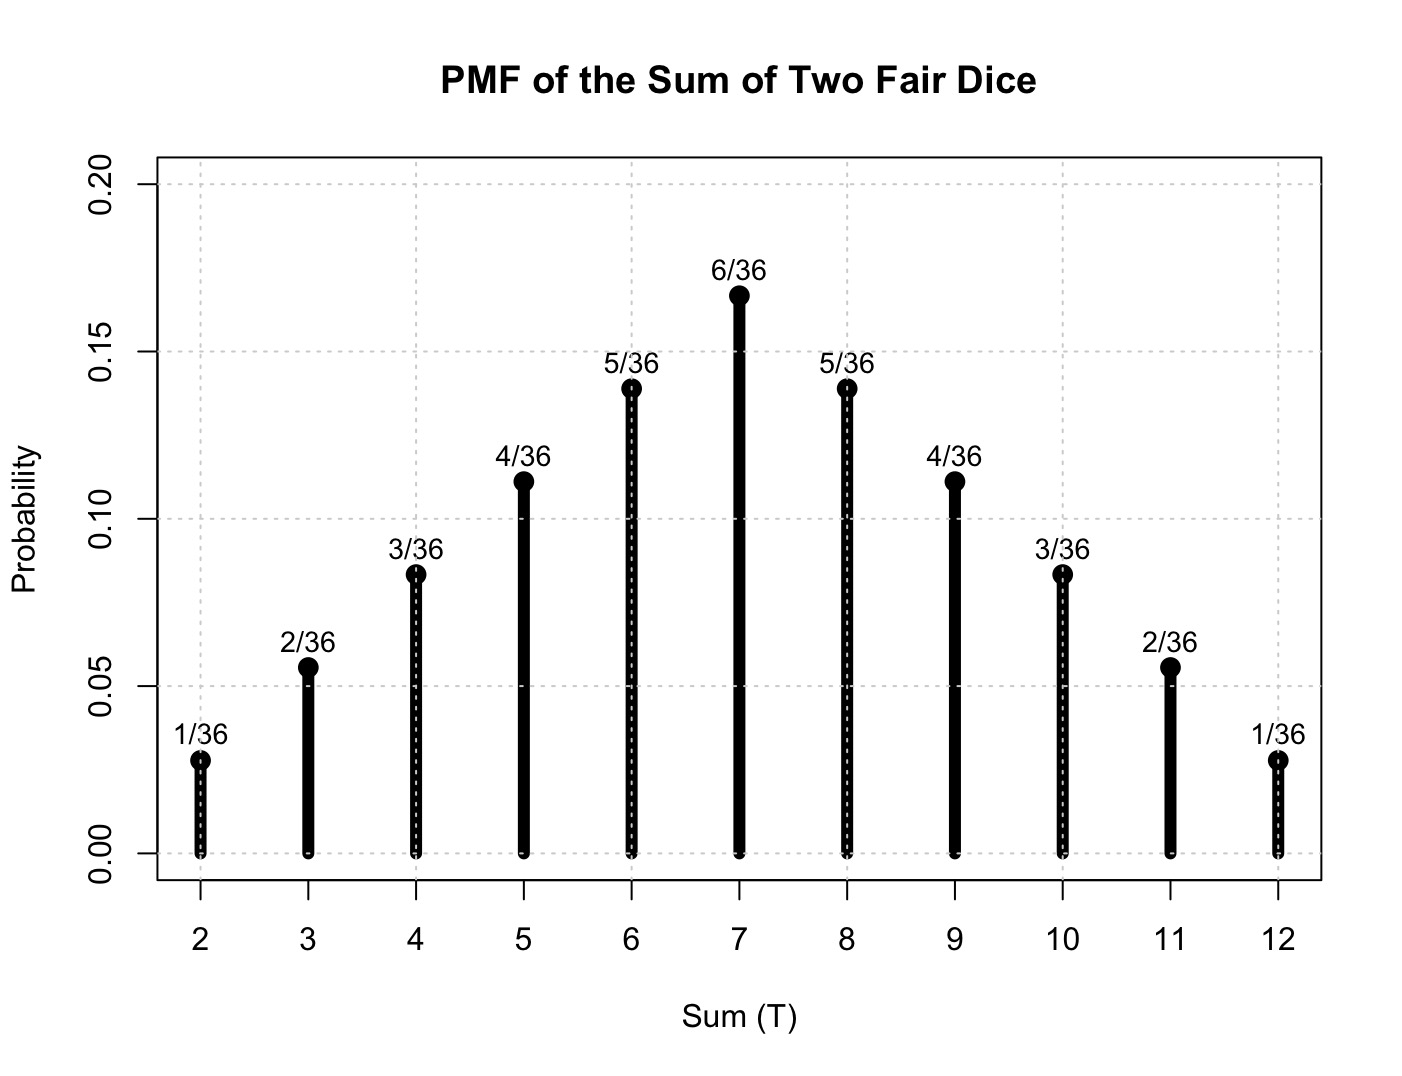
\includegraphics[width=0.5\linewidth]{assets/figures/masssum.jpeg}



\end{frame}








\lecturepart{Named Distributions}






\begin{frame}{Bernoulli Distribution}

\small

A Bernoulli random variable models the outcome of a binary experiment: $\text{success} \leftrightarrow 1,
\qquad
\text{failure} \leftrightarrow 0.$

\begin{keybox}{Bernoulli PMF}
A random variable \(X\) has the Bernoulli distribution with parameter \(0\leq p\leq 1\), written $X\sim\operatorname{Ber}(p),
$
if its PMF is given by
\[
p_X(x)
=
\begin{cases}
p,&x=1,\\
1-p,&x=0,\\
0,&\text{otherwise},
\end{cases}
\]
\end{keybox}

\textbf{Interpretation}: $\Prob(\text{success})=\Prob(X=1)=p,
\qquad
\Prob(\text{failure})=\Prob(X=0)=1-p.$
\vspace{3mm}
\textbf{PMF verification}: Since $0\le p\le1,$, we have $p_X(x)\ge0.$ Also,
\[
\sum_x p_X(x)
=
p+(1-p)
=
1.
\]
Hence \(p_X(x)\) satisfies the properties of a PMF.
\end{frame}









\begin{frame}{Bernoulli Distribution: PMF}

\begin{columns}[c]

\column{0.45\textwidth}

\begin{center}
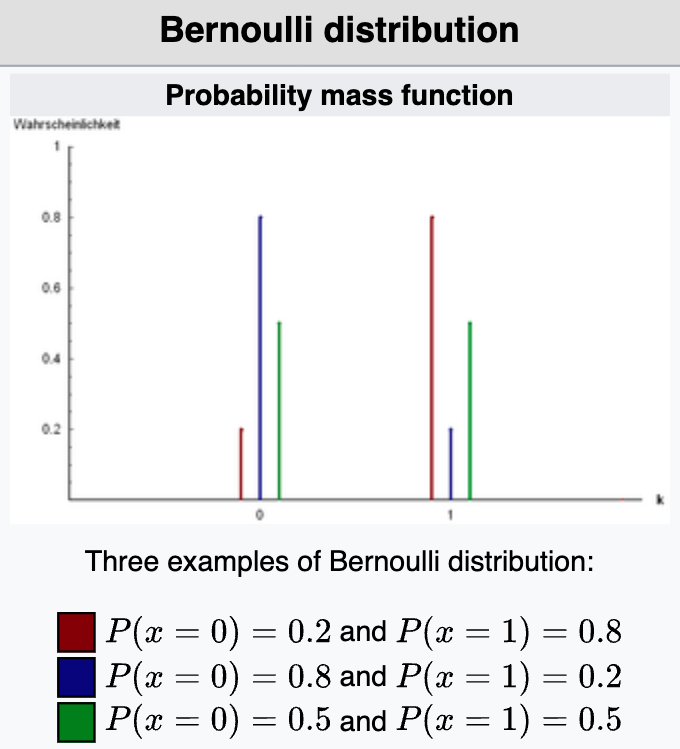
\includegraphics[width=\textwidth]{assets/figures/1.png}
\end{center}

\column{0.55\textwidth}

\[
X\sim \text{Bern}(p),
\]

\[
\Prob(X=1)=p,
\]

\[
\Prob(X=0)=1-p.
\]

\vspace{0.25cm}

A Bernoulli random variable models a single success/failure experiment.

\end{columns}

\end{frame}




\begin{frame}{Binomial Distribution}
\begin{keybox}{Binomial Distribution}
Suppose an experiment consists of 
\begin{itemize}
    \item $n$ independent Bernoulli trials;
    \item where each trial share the same success probability $p$.
\end{itemize}

If $X$ is the number of successes, then

\[
X\sim\text{Bin}(n,p).
\]
\end{keybox}
\end{frame}




\begin{frame}{Binomial PMF}

\small

If
\[
X\sim\operatorname{Bin}(n,p),
\]
then
\[
\boxed{
p_X(k) = \Prob(X=k)
=
\binom{n}{k}
p^k(1-p)^{n-k},
}
\]
for
\[
k=0,1,\dots,n.
\]

\textbf{Interpretation}:
\begin{itemize}
\item \(\binom{n}{k}\): choose which \(k\) trials are successes;
\item \(p^k\): probability of the \(k\) successes;
\item \((1-p)^{n-k}\): probability of the \(n-k\) failures.
\end{itemize}


\textbf{PMF verification}: Since $0\le p\le1,$ we have $p_X(k)\ge0.$
Also,
\[
\sum_{k=0}^n p_X(k)
=
\sum_{k=0}^n
\binom{n}{k}p^k(1-p)^{n-k}
=
(p+(1-p))^n
=
1,
\]
by the Binomial Theorem.

\end{frame}








\begin{frame}{Binomial Distribution: PMF}

\begin{columns}[c]

\column{0.55\textwidth}

\begin{center}
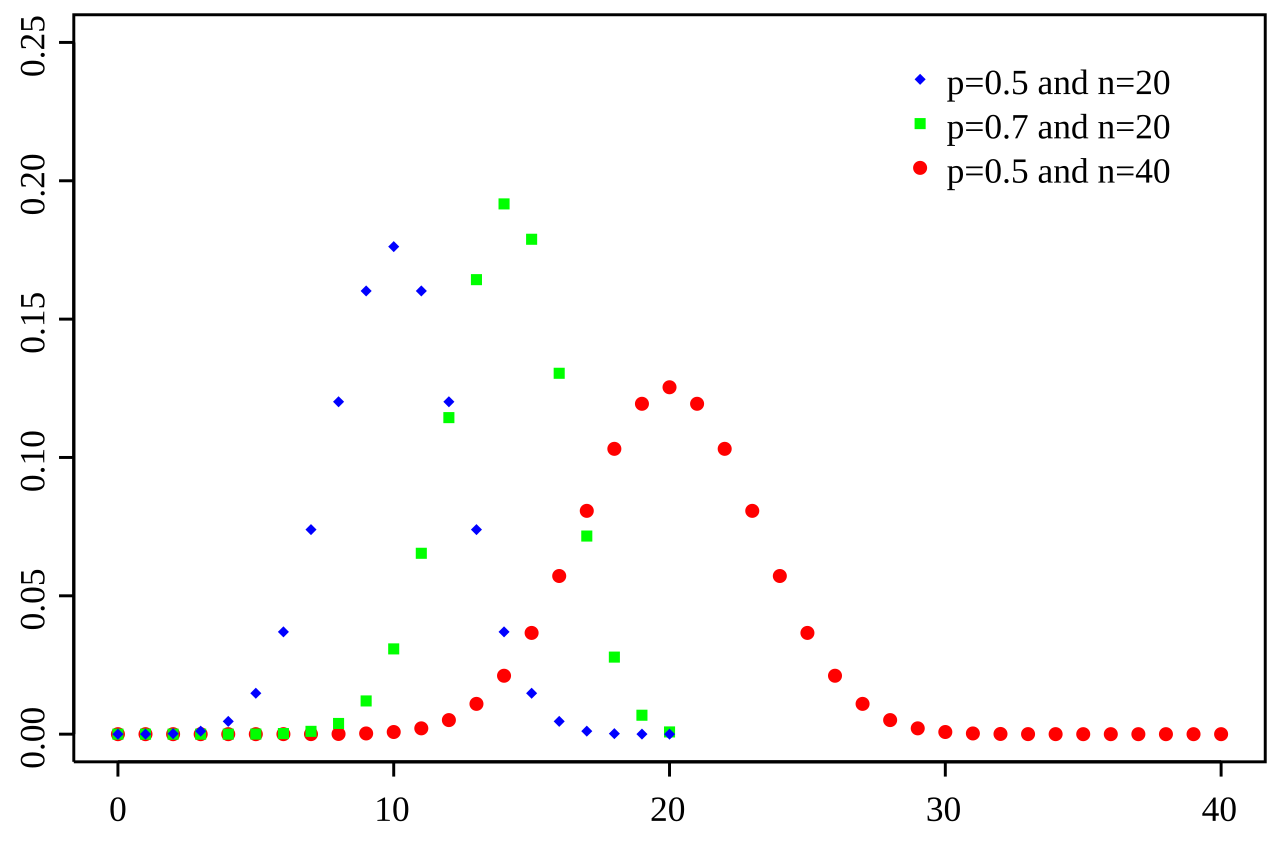
\includegraphics[width=\textwidth]{assets/figures/2.png}
\end{center}

\column{0.40\textwidth}

\[
X\sim \text{Bin}(n,p),
\]

\[
\Prob(X=k)
=
\binom{n}{k}p^k(1-p)^{n-k}.
\]

\end{columns}
Binomial distribution counts the number of successes in $n$ independent Bernoulli trials.

\end{frame}














\begin{frame}{Example: Coin Tosses}
Flip a fair coin $10$ times.

Let:
\[
X=\text{number of Heads}.
\]

Then,
\[
X\sim\text{Bin}(10,\tfrac12).
\]

\vspace{0.25cm}

For example:

\[
\Prob(X=3)
=
\binom{10}{3}
\left(\frac12\right)^{10}.
\]
\end{frame}


\begin{frame}{Geometric Distribution}
\begin{keybox}{Geometric Distribution}
Suppose independent Bernoulli trials are repeated until the first success occurs.

Let
\[
X=\text{number of trials until the first success}.
\]

If each trial share the same success probability $p$, then

\[
X\sim\text{Geom}(p).
\]
\end{keybox}

\vspace{0.25cm}

Possible values:
\[
1,2,3,\dots \ \ \text{(i.e., all positive integers)}
\]

\vspace{0.25cm}

Interpretation:
\begin{itemize}
    \item $X=1$ means success on the first trial;
    \item $X=2$ means failure then success;
    \item $X=3$ means two failures then success;
    \item etc.
\end{itemize}
\end{frame}

















\begin{frame}{Geometric PMF}

\small



\begin{tcolorbox}[
enhanced,
colback=white,
colframe=blue!70!black,
drop shadow,
arc=2mm,
boxrule=0.8pt
]
If
\[
X\sim\operatorname{Geom}(p),
\]
then
\[
\boxed{
\Prob(X=k)
=
(1-p)^{k-1}p,
}
\]
for
\[
k=1,2,3,\dots
\]
\end{tcolorbox}





\textbf{Interpretation}:
\begin{itemize}
\item the first \(k-1\) trials must fail;
\item the \(k\)-th trial must succeed.
\end{itemize}

Hence,
\[
\Prob(X=k)
=
\underbrace{(1-p)^{k-1}}_{\text{failures}}
\underbrace{p}_{\text{success}}.
\]

\textbf{PMF verification}: Since $0\le p\le1,
$ we have $p_X(x)\ge0.$
Also,
\[
\sum_{k=1}^{\infty}p_X(k)
=
\sum_{k=1}^{\infty}(1-p)^{k-1}p
=
p\sum_{k=0}^{\infty}(1-p)^k=p\times\frac{1}{1-(1-p)}
=
p\times \frac1p = 1,
\]
using the geometric sequence formula.

\end{frame}






\begin{frame}{Geometric Distribution: PMF}

\begin{columns}[c]

\column{0.55\textwidth}

\begin{center}
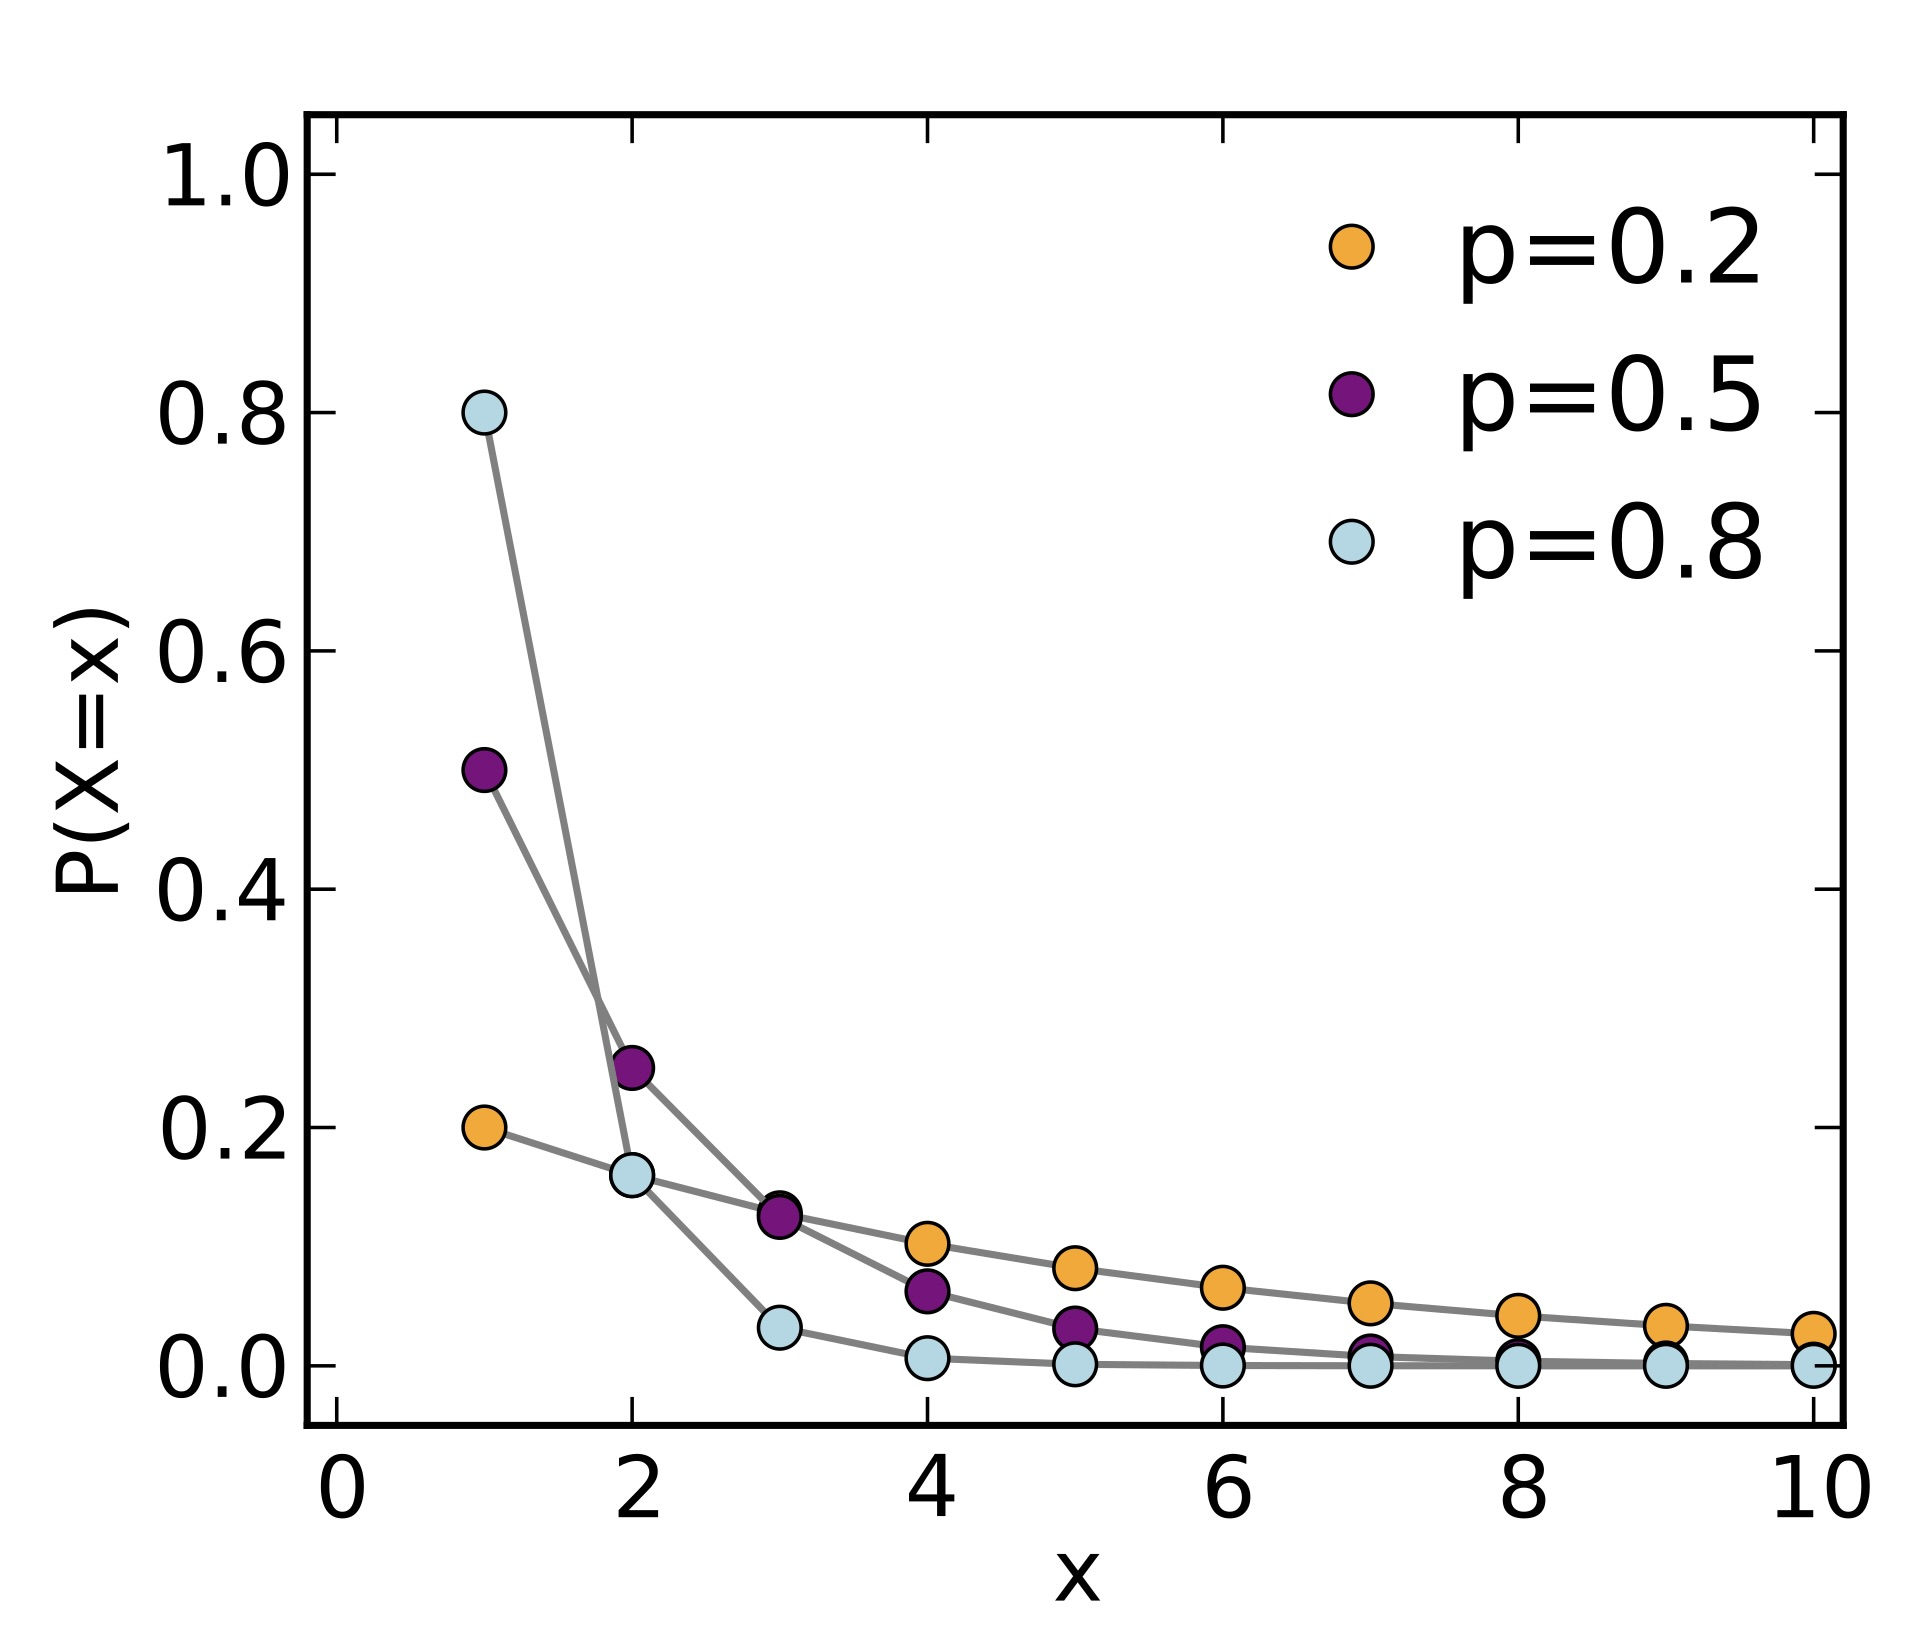
\includegraphics[width=0.95\textwidth]{assets/figures/3.jpeg}
\end{center}

\column{0.40\textwidth}

\[
X\sim \text{Geom}(p),
\]

\[
p_X(x) = \Prob(X=k)
=
(1-p)^{k-1}p,
\]

\[
k=1,2,3,\dots
\]
\end{columns}
The Geometric distribution models the waiting time until the first success.

\end{frame}







\begin{frame}{Memoryless Property of $Geom(p)$ }
The Geometric distribution is the \textbf{only discrete distribution} that satisfies the \textbf{memoryless property}. We will see the continuous counterpart (exponential distribution) in Chapter 5b.

\[
\boxed{
\Prob(X>m+n \mid X>m)
=
\Prob(X>n).
}
\]

\vspace{0.25cm}

Interpretation:

\vspace{0.15cm}

If the first $m$ trials were all failures, the process probabilistically restarts from scratch.

\vspace{0.25cm}

Example:
\[
\Prob(X>10 \mid X>7)
=
\Prob(X>3).
\]

\vspace{0.25cm}

The past failures do not affect future waiting times.
\end{frame}









\begin{frame}{Negative Binomial Distribution}
\begin{keybox}{Negative Binomial Distribution}
Suppose independent Bernoulli trials are repeated until the $r$th success occurs.

Let
\[
X=\text{number of trials needed to obtain } r \text{ successes}.
\]

If each trial has success probability $p$, then

\[
X\sim\text{NegBin}(r,p).
\]
\end{keybox}

\vspace{0.25cm}

Possible values:
\[
r,r+1,r+2,\dots
\]

\vspace{0.25cm}

Interpretation:
\begin{itemize}
    \item the experiment stops once the $r$th success appears;
    \item Geometric distribution is the special case
    \[
    r=1.
    \]
\end{itemize}
\end{frame}











\begin{frame}{Negative Binomial PMF}

\small



\begin{tcolorbox}[
enhanced,
colback=white,
colframe=blue!70!black,
drop shadow,
arc=2mm,
boxrule=0.8pt
]
If
\[
X\sim\operatorname{NegBin}(r,p),
\]
then
\[
\boxed{
p_X(k) = \Prob(X=k)
=
\binom{k-1}{r-1}
p^r(1-p)^{k-r},
}
\]
for
\[
k=r,r+1,r+2,\dots
\]
\end{tcolorbox}












\textbf{Interpretation}:
\begin{itemize}
\item among the first \(k-1\) trials, there must be exactly \(r-1\) successes;
\item the \(k\)-th trial must be a success.
\end{itemize}

Thus,
\[
\Prob(X=k)
=
\underbrace{\binom{k-1}{r-1}}_{\text{arrange first }r-1\text{ successes}}
\underbrace{p^r}_{r\text{ successes}}
\underbrace{(1-p)^{k-r}}_{k-r\text{ failures}}.
\]

\textbf{PMF verification}: Since $0\le p\le1,$ we have $p_X(x)\ge0.
$
\end{frame}



\begin{frame}{PMF verification (conitnue)}
    \[
\sum_{k=r}^{\infty}p_X(k)
=
\sum_{k=r}^{\infty}
\binom{k-1}{r-1}
p^r(1-p)^{k-r}.
\]

Let
\[
j=k-r.
\]
Then \(k=j+r\), so
\[
\sum_{k=r}^{\infty}p_X(k)
=
p^r
\sum_{j=0}^{\infty}
\binom{j+r-1}{r-1}
(1-p)^j.
\]

Using the  \href{https://mathworld.wolfram.com/NegativeBinomialSeries.html}{negative binomial series} identity,
\[
\sum_{j=0}^{\infty}
\binom{j+r-1}{r-1}
x^j
=
\frac{1}{(1-x)^r},
\qquad |x|<1,
\]
with \(x=1-p\), we get
\[
\sum_{k=r}^{\infty}p_X(k)
=
p^r
\frac{1}{(1-(1-p))^r}
=
p^r\frac1{p^r}
=
1.
\]
\end{frame}









\begin{frame}{Understanding the Formula}
To have
\[
X=k,
\]
the following must happen:

\vspace{0.25cm}

\begin{enumerate}
    \item In the first $k-1$ trials, $r-1$ successes must occur.
    \item The final trial must be a success.
\end{enumerate}

\vspace{0.25cm}

Number of ways:
\[
\binom{k-1}{r-1}.
\]

\vspace{0.25cm}

Probability of each arrangement:
\[
p^{\,r-1}(1-p)^{k-r}\cdot p
=
p^r(1-p)^{k-r}.
\]

\vspace{0.25cm}

Multiplying gives:
\[
\Prob(X=k)
=
\binom{k-1}{r-1}
p^r(1-p)^{k-r}.
\]

Note that both the formula and the definition implies that the Negative Binomial distribution is a generalization of the Geometric distribution (when $r=1$, Negative Binomial reduces to Geometric).
\end{frame}

\begin{frame}{Example: Third Heads}
Flip a fair coin repeatedly.

Let
\[
X=\text{number of tosses needed to obtain 3 Heads}.
\]

Then,
\[
X\sim\text{NegBin}(3,\tfrac12).
\]

\vspace{0.25cm}

For example,

\[
\Prob(X=5)
=
\binom{4}{2}
\left(\frac12\right)^3
\left(\frac12\right)^2.
\]

\vspace{0.25cm}

Interpretation:
\begin{itemize}
    \item among the first $4$ tosses, exactly $2$ must be Heads;
    \item the $5$th toss must also be Heads.
\end{itemize}


\end{frame}


\begin{frame}{Geometric vs. Negative Binomial}
\begin{center}
\renewcommand{\arraystretch}{1.4}
\begin{tabular}{ccc}
\toprule
Distribution & Stops After & Support \\
\midrule
Geometric & first success & $1,2,3,\dots$ \\
Negative Binomial & $r$th success & $r,r+1,\dots$ \\
\bottomrule
\end{tabular}
\end{center}

\vspace{0.35cm}

\begin{keybox}{Key Relationship}
The Geometric distribution is a special case of the Negative Binomial distribution:
\[
\text{Geom}(p)=\text{NegBin}(1,p).
\]
\end{keybox}
\end{frame}





































\begin{frame}{Hypergeometric Distribution}
\begin{keybox}{Hypergeometric Story}
An urn contains:
\begin{itemize}
    \item $w$ white balls,
    \item $b$ black balls.
\end{itemize}

Sample $n$ balls without replacement.

If $X$ is the number of white balls selected, then

\[
X\sim\text{HGeom}(w,b,n).
\]
\end{keybox}
\end{frame}







\begin{frame}{Hypergeometric PMF}

\small


\begin{tcolorbox}[
enhanced,
colback=white,
colframe=blue!70!black,
drop shadow,
arc=2mm,
boxrule=0.8pt
]
If
\[
X\sim\operatorname{HGeom}(w,b,n),
\]
then
\[
\boxed{
\Prob(X=k)
=
\frac{
\binom{w}{k}
\binom{b}{n-k}
}{
\binom{w+b}{n}
}.
}
\]

The possible values are
\[
\max(0,n-b)\le k\le \min(w,n).
\]
\end{tcolorbox}


\textbf{Interpretation}:
\begin{itemize}
\item choose \(k\) white balls from the \(w\) white balls;
\item choose \(n-k\) black balls from the \(b\) black balls;
\item divide by the totral number of samples of size \(n\).
\end{itemize}

Thus,
\[
\Prob(X=k)
=
\frac{
\underbrace{\binom{w}{k}}_{\text{choose white balls}}
\underbrace{\binom{b}{n-k}}_{\text{choose black balls}}
}{
\underbrace{\binom{w+b}{n}}_{\text{all samples of size }n}
}.
\]

\vspace{0.1cm}

\textbf{PMF verification}: Since binomial coefficients are nonnegative,
\[
\Prob(X=k)\ge0.
\]
Also,
\[
\sum_k \Prob(X=k)
=
\sum_k
\frac{
\binom{w}{k}\binom{b}{n-k}
}{
\binom{w+b}{n}
}
=
1,
\]
by Vandermonde's identity:
\[
\sum_k
\binom{w}{k}\binom{b}{n-k}
=
\binom{w+b}{n}.
\]

\end{frame}







\begin{frame}{Hypergeometric Distribution: PMF}

\begin{columns}[c]

\column{0.50\textwidth}

\begin{center}
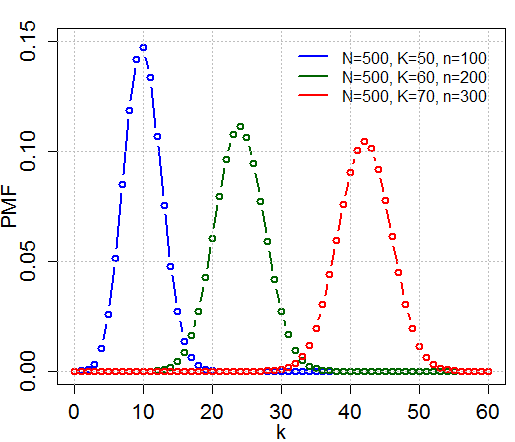
\includegraphics[width=\textwidth]{assets/figures/4.png}
\end{center}

\column{0.40\textwidth}

\[
X\sim \text{HGeom}(w,b,n),
\]

\[
\Prob(X=k)
=
\frac{
\binom{w}{k}
\binom{b}{n-k}
}{
\binom{w+b}{n}
}.
\]
The Hypergeometric distribution arises from sampling without replacement.
\end{columns}
\end{frame}






\begin{frame}{Discrete Uniform Distribution}
\begin{keybox}{Discrete Uniform}
Choose one value uniformly from a finite set $C$.

Then,
\[
X\sim\text{DUnif}(C).
\]
\end{keybox}

\vspace{0.25cm}

All values are equally likely.

\vspace{0.25cm}

Example:
\[
X\sim\text{DUnif}(\{1,2,\dots,6\}).
\]
\end{frame}

\begin{frame}{Poisson Distribution}

\small

\begin{keybox}{Poisson Distribution}
A random variable \(X\) has the Poisson distribution with parameter \(\lambda>0\) if
\[
\Prob(X=k)
=
e^{-\lambda}\frac{\lambda^k}{k!},
\qquad
k=0,1,2,\dots.
\]

Notation:
\[
X\sim \operatorname{Pois}(\lambda).
\]
\end{keybox}

Poisson random variables often model counts of rare events.

\vspace{0.1cm}

\textbf{PMF verification}: Since
\[
\lambda>0,
\]
we have
\[
\Prob(X=k)\ge0.
\]
Also,
\[
\sum_{k=0}^{\infty}p_X(k)
=
\sum_{k=0}^{\infty}
e^{-\lambda}\frac{\lambda^k}{k!}
=
e^{-\lambda}
\sum_{k=0}^{\infty}\frac{\lambda^k}{k!}.
\]
Using the exponential series,
\[
\sum_{k=0}^{\infty}\frac{\lambda^k}{k!}
=
e^\lambda,
\]
Hence \(\Prob(X=k)\) satisfies the properties of a PMF.

\end{frame}







\begin{frame}{Poisson Distribution: PMF}

\begin{columns}[c]

\column{0.50\textwidth}

\begin{center}
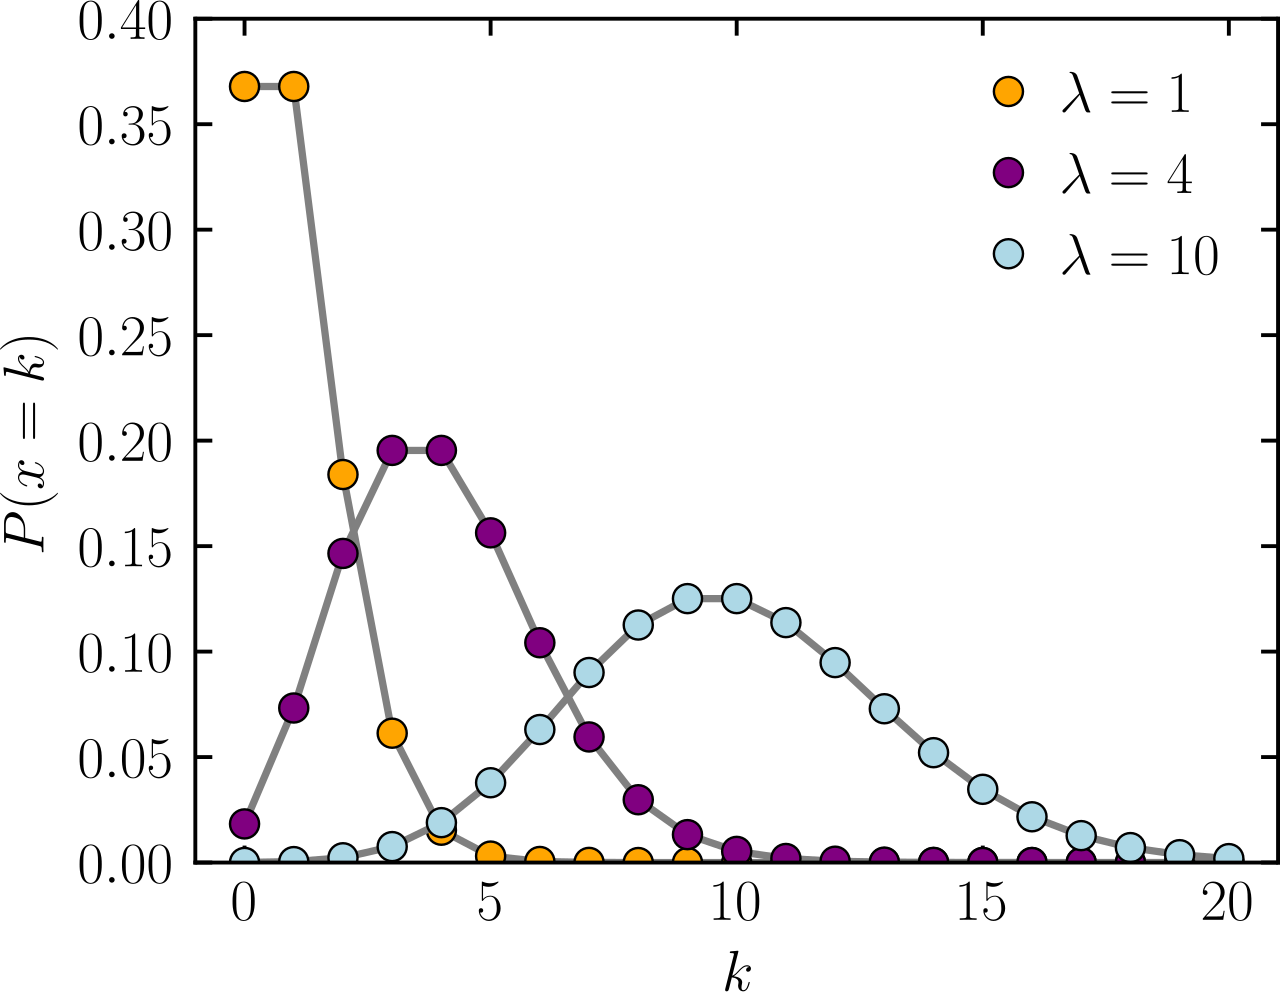
\includegraphics[width=\textwidth]{assets/figures/6.png}
\end{center}

\column{0.40\textwidth}

\[
X\sim Pois(\lambda),
\]

\[
\Prob(X=k)
=
e^{-\lambda}
\frac{\lambda^k}{k!},
\qquad
k=0,1,2,\dots
\]

\vspace{0.25cm}

The Poisson distribution models the number of events occurring in a fixed interval of time or space.

\vspace{0.2cm}

Typical examples include:
\begin{itemize}
    \item phone calls arriving,
    \item radioactive decays,
    \item website visits,
    \item accidents in a day.
\end{itemize}

\end{columns}

\end{frame}






















\lecturepart{CDFs}

\begin{frame}{Cumulative Distribution Functions}
\begin{keybox}{Definition}
The cumulative distribution function (CDF) of $X$ is

\[
\boxed{
F_X(x)=\Prob(X\leq x) .
}
\]
\end{keybox}

\vspace{0.25cm}

\begin{itemize}
    \item The CDF accumulates all the probability mass that exists from $-\infty$ to (inclusive) $x$. 

\item In other words, $F_X(x) = \Prob(X \in (-\infty, x]) = \Prob(-\infty < X\leq x)$ are three different ways of introducing the same thing, the CDF of $X$ at point $x$.

\item Note that $X\leq x$ (or $X\in (- \infty, x],$ or $-\infty < X\leq x),$  actually refer to an EVENT:
\begin{equation*}
    \{X\leq x\} = \{ s \in \Sample \ : \ X(s)\leq x  \}  = X^{-1}((-\infty , x]))
\end{equation*}

\item In general, $\{X \in A \} = \{ s\in \Sample \ : \ X(s) \in A \} = X^{-1}(A)$
    
\end{itemize}
\end{frame}

\begin{frame}{PMF vs. CDF}
For discrete random variables:

\vspace{0.25cm}

\begin{itemize}
    \item PMF:
    \[
    p_X(x) = \Prob(X=x)
    \]

    gives probability at one point;

    \item CDF:
    \[
   F_X(x) =  \Prob(X\leq x)
    \]

    gives cumulative probability.
\end{itemize}

\vspace{0.25cm}

The CDF is increasing and ranges from $0$ to $1$.
\end{frame}



\begin{frame}{Properties of a CDF}

\begin{columns}[T]

\begin{column}{0.38\textwidth}

\begin{keybox}{Key properties}
Every CDF satisfies:
\begin{itemize}
    \item $0 \le F(x)\le 1,$

    \item $F(x)$ is increasing,

    \item $\displaystyle \lim_{x\to -\infty}F(x)=0,$

    \item $\displaystyle \lim_{x\to \infty}F(x)=1.$
\end{itemize}
\end{keybox}

\end{column}

\begin{column}{0.62\textwidth}

\begin{center}
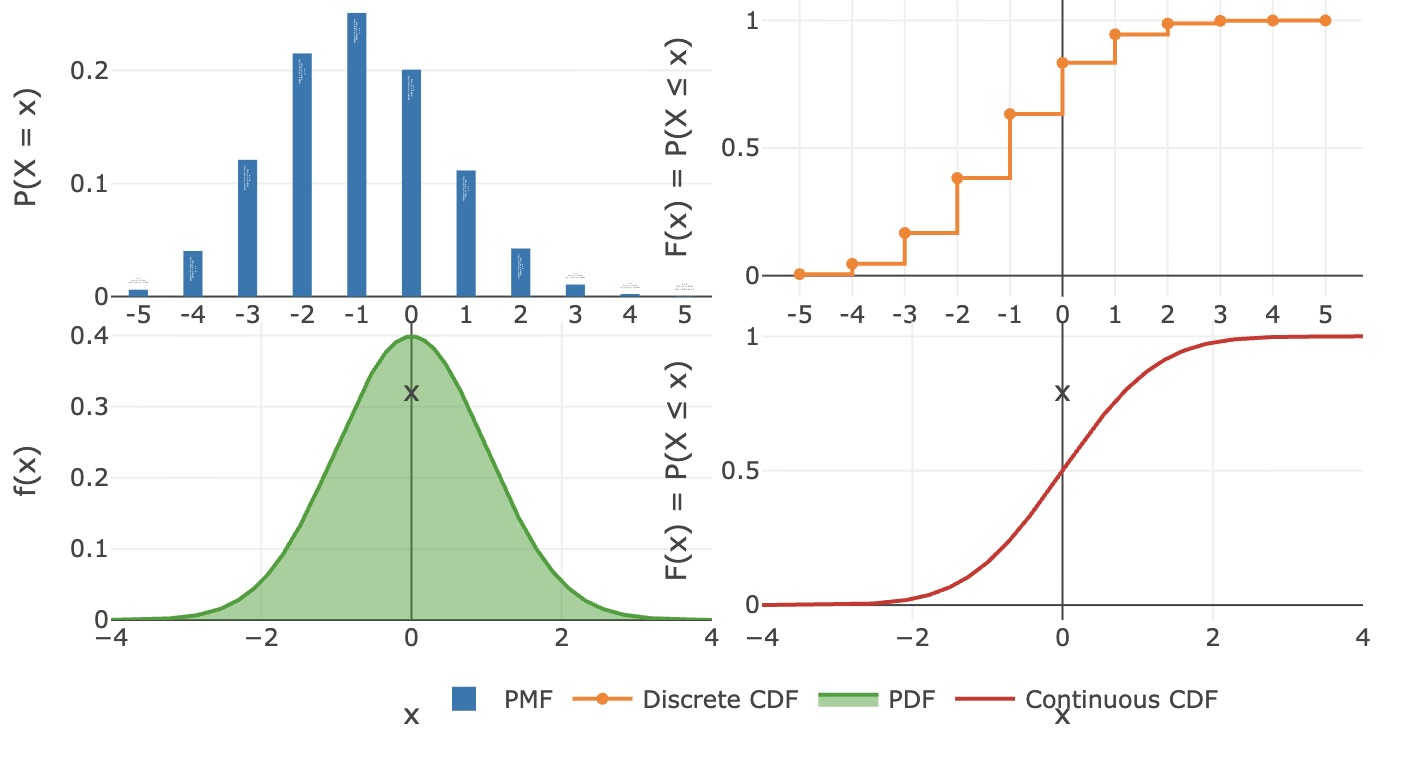
\includegraphics[width=\textwidth]{assets/figures/pdfpmf.jpeg}

\vspace{0.05cm}

{\scriptsize
\href{https://armanjg.github.io/MATH-394-Probability-1-v2/Figures/pdfpmf.html}
{Interactive visualization of PMF/PDF and CDF accumulation.}
}
\end{center}

\end{column}

\end{columns}

\end{frame}



\lecturepart{Functions of Random Variables}

\begin{frame}{Functions of Random Variables}
If $X$ is a random variable and
\[
g:\mathbb{R}\to\mathbb{R},
\]
then

\[
Y = g(X)
\]

is also a random variable.

\vspace{0.25cm}

Examples:
\[
Y = X^2,
\qquad
Y = \sqrt{X},
\qquad
Y = |X|,
\qquad
Y = 2X+1.
\]

Question: How to find $F_{Y}(y)$? We will see later in Transformations of r.v.s.
\end{frame}



\begin{frame}{Several Random Variables on One Space}
Different random variables may be defined on the same experiment.

\vspace{0.25cm}

Example:
\begin{itemize}
    \item $X$ = first die $\in \set{1,2,3,4,5,6}$;
    \item $Y$ = second die $\in \set{1,2,3,4,5,6}$;
    \item $X+Y$ = total $\in \set{1,2,\dots, 11,12}$;
    \item $\max(X,Y)$ = maximum $\in \set{1,2,3,4,5,6}$;
    \item $|X-Y|$ = difference $\in \set{0,1,2,3,4,5}$;
\end{itemize}

\vspace{0.25cm}

Each gives a different numerical summary of the same experiment.
\end{frame}

\begin{frame}{Summary}
\begin{itemize}
    \item A random variable is a function from the sample space to $\mathbb{R}$.

    \item Discrete random variables are described by PMFs.

    \item Important distributions:
    \[
    \text{Bernoulli},\quad
    \text{Binomial},\quad
    \text{Hypergeometric},\quad
    \text{Discrete Uniform}.
    \]

    \item CDFs accumulate probability:
    \[
    F_X(x)=\Prob(X\leq x).
    \]

    \item Functions of random variables are themselves random variables.

    \item Random variables help convert complicated experiments into manageable numerical objects.
\end{itemize}

\vspace{0.25cm}

\begin{keybox}{Next lecture}
Expectation
\end{keybox}
\end{frame}